\documentclass[12pt,a4paper]{article}
\usepackage[utf8]{inputenc}
\usepackage[spanish]{babel}

% Paquetes

\usepackage{amsmath}
\usepackage{amsfonts}
\usepackage{amssymb}
\usepackage{amsthm}  % Permite crear teoremas nuevos / Estilos de teoremas 

\usepackage{chngcntr}
\usepackage{graphicx} % 
\usepackage[colorlinks=true,allcolors=blue]{hyperref} % Crea las hiperreferencias (clicas y te mueves)
\graphicspath{{Figuras/}}
\usepackage{fancybox} % para usar la caja de los ejemplos

% Autor y titulo

\title{Práctica Efecto Fotoélectrico}
\author{Daniel Vázquez Lago}

% Forma del  texto

\setlength{\parindent}{15px}
\usepackage[left=2.25cm,right=2cm,top=4cm,bottom=2cm]{geometry}

% Otros


\numberwithin{equation}{section}
\numberwithin{table}{section}
\numberwithin{figure}{section}

% Comandos propios
\newcommand{\tquad}{\quad \quad \quad}

\newcommand{\parentesis}[1]{\left( #1  \right)}
\newcommand{\parciales}[2]{\frac{\partial #1}{\partial #2}}
\newcommand{\pparciales}[2]{\parentesis{\parciales{#1}{#2}}}
\newcommand{\ccorchetes}[1]{\left[ #1  \right]}
\newcommand{\D}{\mathrm{d}}
\newcommand{\derivadas}[2]{\frac{\D #1}{\D #2}}
\newcommand{\cte}{\mathrm{cte}}

\newcommand{\Tr}{\mathrm{Tr} \ }


\newcommand{\eup}{\mid \uparrow \rangle}
\newcommand{\edw}{\mid \downarrow \rangle}

\newcommand{\Hcal}{\mathcal{H}}
% Comandos vectoriales

\newcommand{\xn}{\mathbf{x}}
\newcommand{\yn}{\mathbf{y}}
\newcommand{\zn}{\mathbf{z}}
\newcommand{\vn}{\mathbf{v}}
\newcommand{\un}{\mathbf{u}}
\newcommand{\rn}{\mathbf{r}}
\newcommand{\qn}{\mathbf{q}}
\newcommand{\pn}{\mathbf{p}}
\newcommand{\kn}{\mathbf{k}}
\newcommand{\sn}{\mathbf{s}}
\newcommand{\an}{\mathbf{a}}
\newcommand{\bn}{\mathbf{b}}
\newcommand{\nn}{\mathbf{n}}

\newcommand{\rhon}{\mathbf{\rho}}


\newcommand{\An}{\mathbf{A}}
\newcommand{\Pn}{\mathbf{P}}
\newcommand{\Bn}{\mathbf{B}}
\newcommand{\Sn}{\mathbf{S}}
\newcommand{\En}{\mathbf{E}}
\newcommand{\Hn}{\mathbf{H}}
\newcommand{\Encal}{\boldsymbol{\mathcal{E}}}
\newcommand{\mun}{\boldsymbol{\mu}}


% Comandos vectoriales unitarios

\newcommand{\hrho}{\hat{\rhon}}
\newcommand{\hnu}{\hat{\un}}
\newcommand{\hns}{\hat{\sn}}
\newcommand{\hnr}{\hat{\rn}}
\newcommand{\hnx}{\hat{\xn}}
\newcommand{\hny}{\hat{\yn}}
\newcommand{\hnz}{\hat{\zn}}

% Comandos teoremas

\newtheorem{theorem}{Teorema}[section]
%\theoremstyle{definition}
\newtheorem{definition}{Definicion}[section]

\begin{document}

\maketitle

\newpage

\tableofcontents

\newpage

\section{Objetivos}

El objetivo principal de esta práctica es obtener la constante de Planck $h$, la función de trabajo de una fotocélula $W$  y la frecuencia umbral $\nu_0$ (siendo esta última una función de las dos primeras). Este es la principal finalidad de la práctica. \\


\section{Introducción teórica}

Para calcular la constante de Planck usaremos el efecto fotoeléctrico (tal y como indica el nombre de la práctica). El efecto fotoeléctrico describe con precisión el fenómeno de arrancar electrones de la superficie de un metal cuando es iluminada, siempre y cuando se verifiquen determinadas condiciones. Si $\nu$ es la frecuencia de la luz, la energía cinética máxima ($T_{max}$) con la que podemos arrancar los electrones de dicho material viene determinada por

\begin{equation}
T_{max} = h \mu - W \label{Ec:2.1}
\end{equation}
donde $W$ es una constante de cada material llamada la \textbf{función de trabajo}. Cuando $h \nu < W$ simplemente no se arrancan electrones del átomo. Definimos la frecuencia umbral $\nu_0$ como la frecuencia a partir la cual el efecto eléctrico aparece. Esto es:

\begin{equation}
\nu_0 = \frac{W}{h}
\end{equation}
Con esto ya podemos hacernos una idea de que vamos a usar en esta práctica: si fuéramos capaces de obtener $T_{\max}$ de alguna manera, simplemente haciendo una regresión que enfrentase $T$ y $\nu$ podríamos obtener la pendiente (con la cuál obtener $h$) y el término independiente (con el que obtener $W$). \\

Entonces lo que haremos será usar una lampara espectral de mercurio, de tal manera que emitiremos fotones con una frecuencia particular muy estrecha (casi-monocromática), que haremos pasar por un filtro que seleccionara una de las líneas espectrales de la lámpara. Tras esto, haremos que la luz filtrada (con una $\lambda$ conocida) incida sobre una célula fotovoltaica.  \\

La célula fotovoltaica nos dará una medida de $T_{max}$. La célula consta de un ánodo y un cátodo. La luz incide en el cátodo, haciendo que el cátodo emita electrones hacia el ánodo. Un amperímetro conectado entre ambos nos dará un valor de la intensidad que de los fotoelectrones que atraviesan la célula. Para obtener la energía máxima lo que haremos será conectar a este circuito un voltaje llamado \textit{voltaje de frenado} $V_f$ de tal manera que reduzca la velocidad de los electrones (por eso mismo su valor es negativo). Si el voltaje de frenado es muy grande este impedirá que los electrones lleguen al ánodo, haciendo que la intensidad que circule sea nula. \\

Si vamos aumentando poco a poco el voltaje (haciéndolo menos negativo), llegará un punto a partir del cual la intensidad comience a aumenta. En este punto los electrones con máxima intensidad habrán llegado al cátodo. Si seguimos aumentando el voltaje incluso aquellos que no tienen energía cinética máxima llegarán al cátodo. Si llamamos $V_0$ al voltaje para el cual la intensidad comienza a aumentar, esto es, a partir la cual los electrones con máxima velocidad llegan al ánodo, tendremos la relación:

\begin{equation}
T_{\max} = eV_0 
\end{equation}
donde $e$ es la carga del electrón constante conocida. Asumiremos un valor $e=1.609\cdot 10^{-19}$ C. Reescribiendo la ecuación \ref{Ec:2.1} en términos de $V_0$ y $\lambda$ tenemos que:

\begin{equation}
V_0 = \frac{h}{e} \frac{c}{\lambda} +  \frac{W}{e}
\end{equation}
siendo $c=3\cdot10^8$ m/s. la velocidad de la luz. Conocidas $V_0$ para determinadas longitudes de onda, si hacemos la regresión lineal $V_0 = \frac{b}{\lambda}+a$, podremos obtener $h$ en función de $b$ y $W$ en función de $a$:

\begin{equation}
b = \frac{c \cdot h}{e} \Longrightarrow h = \frac{e\cdot b}{c} 
\end{equation}
\begin{equation}
a = \frac{W}{e} \Longrightarrow W = e \cdot a
\end{equation}
Una vez hemos entendido como se calcula la constante de Plank (y la función de trabajo), solo tendremos que calcular $V_0$ para cada $\lambda$. Presentamos 3 métodos para calcularlo. El \textbf{método 1} será aproximar abitrariamente el lugar a partir del cual la intensidad comienza a crecer. El \textbf{método 2} se basa, \textit{grosso modo}, en aproximar $I(V)$ a dos rectas y calcular el punto de corte. Dicho punto de corte será $V_0$. El \textbf{método 3} es quizás el más interesante de los 3, y el que mas juego va a dar. En este aproximaremos la curva $I(V)$ a una exponencial con determinados parámetros, para luego calcular $V_0$ a partir de estos. En los siguientes apartados presentaremos los 3. Es necesario decir que, idealmente, los 3 métodos deberían dar el mismo $V_0$ para cada $\lambda$, aunque para sorpresa de nadie, no va a pasar. Será comentado posteriormente.


\subsection{Método 1: aproximación arbitraria} \label{Subsec:2.1}

Este método es el más sencillo de todos. A ojo, veremos el punto a partir del cual nos parece que la intensidad comienza a aumentar, el cual será $V_0$. Así para cada uno de los filtros. A priori puede parecer que no ningún tipo de problema, ni de cálculo ni de comprensión. Sin embargo abre dos debates importantes. \\

El primer problema es que la metodología es muy flexible, lo cuál no puede provocar que falseemos los datos para obtener una constante de Plank más acertada. De hecho puedo seleccionar ``abitrariamente'' unos datos que me den el resultado que quiera. Esto se resolverá seleccionando los puntos antes del estudio de cualquier otro tema, para así no tener una intuición de donde puedan estar (y por tanto elegir con un propósito). \\

El segundo problema viene dado por la incertidumbre del problema. ¿Qué incertidumbre le damos a una medida?¿También es de ``elección libre''?¿Son todas iguales, o serán diferentes? Lo que haremos será ver la región por en la cual sería válido que estuviera el punto de $V_0$, marcar otros posibles puntos, y evaluar la distancia entre estos y el punto asignado como $V_0$. 

\subsection{Método 2: punto de corte}\label{Subsec:2.2}

Este método nos dice que aproximemos la curva $I(V_f)$ a dos rectas: una en la región donde $I$ es mínima y constante, y otra donde $I(V_f)$ crece. El punto de corte será $V_0$. El punto de corte de dos rectas $I=a_1+b_1V_f$ y $I=a_2+b_2 V_f$ vendrá dado por:

\begin{equation}
V_0 = -\frac{a_2-a_1}{b_2-b_1}
\end{equation}
por lo que la incertidumbre de $V_0$ viene determinado por la incertidumbre de todos todos los términos de la regresión. La fórmula de propagación de incertidumbre nos dice que:

\begin{equation}
s(V_0) = \sqrt{\parentesis{\frac{s(a_2)}{b_2-b_1}}^2+\parentesis{\frac{s(a_1)}{b_2-b_1}}^2+\parentesis{\frac{a_2-a_1}{(b_2-b_1)^2}s(b_1)}^2+\parentesis{\frac{a_2-a_1}{(b_2-b_1)^2}s(b_2)}^2} \label{Ec:2.8}
\end{equation}
La pregunta ahora es cual es el método para seleccionar los puntos para los cuales se puede hacer la aproximación. Aunque la selección sea arbitraria (del método), a diferencia de la anterior este método será mucho más sistemático, y por tanto sencillo de implementar. Los puntos que se usaran de ajuste para las intensidades mas bajas serán aquellos que cuya intensidad no supere los $4$ pA respecto la intensidad más baja medida. Los puntos que se usarán de ajuste para las intensidades mas altas será todo punto a partir del primero que verifique un salto de $2 $ pA entre el voltaje $V_i$ e $V_{i+2}$. A partir de este $i$ todos los voltajes empezarán a usarse para dicho ajuste. \\

La elección de los 2 $pA$ puede cambiarse (al igual que la de los $4$ pA, pero es la única forma de poder evaluar correctamente las intensidades para todos los filtros, ya que si usaramos 3 pA no podríamos obtener una recta para el último filtro. Sería muy interesante un estudio sobre cual es la mejor elección y la que arroja el mejor resultado, pero eso sería un estudio a parte en sí mismo, innecesario para lo que queremos hacer en esta práctica.


\subsection{Método 3: exponenciales} \label{Subsec:2.3}

En este método aproximaremos la curva $I(V_f)$ a una curva exponencial con 3 parámetros $A$,$B$ y $C$. En ese caso tenemos que:

\begin{equation}
I = A \parentesis{e^{B(V_f-C)}-1}
\end{equation}
Ahora debemos obtener alguna función de los parámetros que nos de el punto de corte. Una posible medida es la región para la cual $V_0 = C$, ya que en ese caso tendremos que $I$ habrá crecido $A$ (ya que pasa de $-A$ cuando $V_f<<C$ a $0$ cuando $V_f=V_0=C$). En este caso el valor $V_0$ será aquel que verifique $I(V_0) = 0$. Sin embargo podemos ver en las gráficas que $I$ empieza a crecer aun cuando tiene valores negativos. A pesar de sus malos resultados (para nuestros datos), lo usaremos igual, ya que es el método que aparece en gran parte de la literatura y por el guión. Por esta razón le llamaremos a esta versión la \textit{método 3-1}. La incertidumbre para esta versión:

\begin{equation}
s(V_0) = s(C)
\end{equation}

Un nuevo criterio (que arrojará mejores resultados para nuestros datos) podría ser aquel $V_0 = C-1/B$. Esta forma asignaría el valor de la intensidad de $I(V_0)=A(e^{-1}-1)$. Esto es, una intensidad de $I\approx-0.63A$. A esta forma de hacerlo se le llamará la \textit{método 3-2}. Sin embargo esto arroja un nuevo dilema: si podemos crear criterios completamente arbitrarios es obvio que podemos elegir uno que nos de el resultado que queremos, aunque a la hora de la verdad escoger $V_0=C$ puede ser tan ``caprichoso'' como elegir $V_0=C-1/B$. \\


\begin{equation}
s(V_0) = \sqrt{\parentesis{s(C)}^2+\parentesis{\frac{s(B)}{B^2}}^2}
\end{equation}

Por tanto justificaremos esta nueva forma de calcular $V_0$ como un añadido a la práctica (incluso implementable a prácticas posteriores de otros alumnos) en base a los resultados. Teóricamente también se puede justificar, ya que un aumento de $0.47I_0$ siendo $I_0=A$ la intensidad   en el límite $V_f \rightarrow \infty$ es suficiente como para decir que la intensidad ya está creciendo.  \\

\section{Obtención de $V_0$}

Acabamos de explicar como obtendremos los datos de $V_0$ a partir de los pares  $(I,V_f)$. Ahora tenemos que obtenerlos. Lo mas común en esta sección sería presentar cada método, con sus tablas y su gráficas, y comentar un poco el resultado. El problema de está práctica es la gran cantidad de datos manejados. Tenemos que realizar 5 gráficas para cada método (menos el método 1) con 5 datos por método. Siendo realistas explicitar todas las tablas y gráficas aquí solo empeoraría la calidad de la memoria. \\

La única diferencia con otras memorias será que aquí haremos referencias al anexo con las gráficas (\ref{Sec:6-graficas}) y con las tablas (\ref{Sec:7-tablas}) continuamente. Comentaremos sobretodo las incertidumbres obtenidas con cada método, la razón por la cuál son tan grandes (o tan pequeñas) respecto a las demás, para finalmente pasar al gran problema de esta memoria: los datos del primer filtro ($\lambda=340$nm), el cual se suma a los dos objetivos prioritarios ya presentados (calcular $h$,$\nu_0$ y $W$; y demostrar como $V_0 = C-1/B$ en el tercer método es mas fiable). \\

Una breve descripción del problema sería la siguiente: los resultados de $V_0$ para el primer filtro no concuerdan con los demás. Ya hemos dicho que debe seguir una recta tal que $V_0 \varpropto \frac{1}{\lambda}$, sin embargo no es así. Es precisamente por eso por lo que en la sección siguiente nos hemos obligado a calcular todos los términos de $h,W,\mu_0$ usando y no usando dicho valor. Eso multiplicará la complejidad y tamaño de la práctica. 

\subsection{Método 1}

Como hemos comentando en el apartado \ref{Subsec:2.1}, necesitamos explicitar las incertidumbres y los valores de los potenciales. Tal y como podemos ver en las tablas del apartado \ref{Subsec:7.1} no hemos asumido una incertidumbre constante (que es, probablemente, lo mas común en este tipo de problemas). Lo que hicimos es coger el rango para el cual, según nosotros, el que el punto donde \textit{realmente} empieza a crecer se encuentra con un $99\%$. Luego cogimos el punto medio de dicho rango, y asignamos la distancia media de dicho rango como incertidumbre. Dado que dudamos mas en aquellos filtros con mayor longitud de onda, cabe esperar que tengan mas incertidumbre. Esto también ocurre con los otros métodos, por lo que es normal que en este también ocurra, ya que tratamos que sea lo mas objetivo posible. \\

Nos pareció el método más óptimo para elegir el valor y su incertidumbre, ya que de cualquier otro método podríamos ``forzar'' el valor a darnos lo que queríamos. En cualquier caso podemos ver como este método arroja valores parecidos a los demás, lo que nos dice que los siguientes métodos arrojan un valor parecido al que cabría esperar, lo cuál es, ciertamente, bueno. 

\subsection{Método 2}

La incertidumbre de cada dato viene arrojada por la ecuación \ref{Ec:2.8}. Como podemos ver dicha ecuación contiene 4 parámetros diferentes, cada una con una incertidumbre dada por las regresiones lineales. Cuanto antes empiece a crecer, mayor será la incertidumbre de los parámetros de las regresiones. Esto se debe a dos factores: cuanto antes empiece a crecer las regresiones se harán con mas datos, y que cuanto antes empiece a crecer la zona de crecimiento mas se parecerá a una exponencial y no a una recta. Es por esa misma razón que los valores de $s(V_0)$ con mayor $\lambda$ son mayores (entorno a 3-2 veces que los de menor $\lambda$). Este fenómeno se puede ver perfectamente en las gráficas \ref{Fig:6.1.1}, \ref{Fig:6.1.2} y \ref{Fig:6.1.3}, donde a diferencia de las gráficas \ref{Fig:6.1.4} y \ref{Fig:6.1.5}, las líneas que aproximan la zona de crecimiento no son muy buenas. No hemos incluido los parámetros de cada regresión ya que serían 4 datos y 4 incertidumbres por cada filtro. En todas las regresiones se ha incluido el valor del punto de corte $V_0$.

\subsection{Método 3}

Dado que el método 3-2 cuenta con un parámetro mas, la incertidumbre del $V_0$ dado por este será mas grande que el dado por el método 3-1.  Esto se verifica en todas los filtros. Este factor, aunque pueda parecer perjudicial para la demostración de que el método 3-2 es peor, en realidad es ventajoso. El método 3-1 solo tiene en cuenta uno de los parámetros usados en la regresión, por lo que modificar un varios datos no alterará gravemente el resultado, mientras que el método 3-2 si será mucho mas sensible. De este modo el método 3-2 nos puede decir con mayor precisión cuando, en el proceso de tomar datos, estamos cometiendo un error de medida. De este modo si usando el método 3-2 el resultado final se parece mas al esperado, tendremos que será un indicativo de que las cosas se han hecho bien, o al menos arroja mas información que el método 3-1. \\

Como podemos ver aquellas regresiones exponenciales que peor cuadren con los datos (\ref{Fig:6.2.2}, \ref{Fig:6.2.5}) son las que mas incertidumbre tienen (véase tablas \ref{Subsec:7.1}, a diferencia de las regresiones de las figuras \ref{Fig:6.2.1},  \ref{Fig:6.2.3} y \ref{Fig:6.2.4}. La razón por la cual la regresión $\lambda =405$nm se ajuste peor a los datos es completamente diferente a la de la regresión $\lambda =580$nm. Para la primera exponencial es la cantidad de datos (entorno a 210, a diferencia de las demás que rondan los 120-160) lo que provoca esto. Para la exponencial de 580nm es lo lento y tarde que empieza a crecer lo que hace que los parámetros no se acaben por adaptar bien a los datos. A pesar de cambiar varias veces los parámetros iniciales en el curvefit de scipy (librería python), no fuimos capaces de mejorar el ajuste, por lo que decidimos dejarlo así. 

\section{Comparación de las pendientes}
 
La constante de Planck se calcula a partir de la pendiente de las regresiones lineales, por lo que la incertidumbre de está última es proporcional a la primera. En el guion se nos pide que comparemos nuestras pendientes con el valor de la pendiente esperada. Por esta misma razón podemos ver que en todas las figuras (\ref{Fig:6.3.1}, \ref{Fig:6.3.1}, \ref{Fig:6.4.1}, \ref{Fig:6.4.2}, \ref{Fig:6.5.1}, \ref{Fig:6.5.2}, \ref{Fig:6.5.3}, \ref{Fig:6.5.4}) hemos incluido los valores de la pendiente y el coeficiente independiente, aunque sin su incertidumbre. Para poder hacer una mejor comparación incluimos la siguiente tabla (siendo $b_1$ la pendiente usando el primer filtro y $b_2$ sin usar el primer filtro):

\begin{table}[h!] \centering 
\begin{tabular}{c|c|c|c|c} 
 & $b_{1}$ (kV$\cdot$nm) & $s(b_{1})$ (kV$\cdot$nm) & $b_{2}$ (kV$\cdot$nm) & $s(b_{2})$ (kV$\cdot$nm) \\ \hline 
Metodo 1  & 0.82  & 0.15 & 0.98  & 0.13  \\ 
Metodo 2  & 1.03  & 0.22 & 1.23  & 0.27  \\ 
Metodo 3-1  & 0.39  & 0.28 & 0.75  & 0.23  \\ 
Metodo 3-2  & 0.86  & 0.29 & 1.13  & 0.15  \\ 
\end{tabular}\caption{tabla de las pendientes para cada método.} 
\label{Tab:00} 
\end{table} 

Donde el valor tabulado es 1.239 kV$\cdot$nm. Como podemos ver mayor parte de los valores de la pendiente distan bastante del valor tabulado, exceptuando $b_2$ para el método 2, donde la diferencia es completamente mínima. Otros $b_2$ también se acercan al valor nominal, tales como el método 3-2 y método 1; así como el $b_1$ del método 2. \\

Las incertidumbres de las pendientes $b_1$ son mucho mayores, debido a que el primer dato es un dato muy desviado respecto los otros. En las figuras se puede ver como los datos, aunque si siguen un crecimiento lineal, lo hacen separándose bastante de la regresión, por lo que las incertidumbres acaban siendo moderadamente altas. Aquellas donde la regresión lineal se ajusta mejor ( \ref{Fig:6.2.1}, \ref{Fig:6.5.4}) la incertidumbre es mucho menor. En el apartado de conclusiones ya comentaremos los valores de $h$ comparándolos con el valor nominal. 

\section{Discusión de resultados y conclusión}

\subsection{Eliminación del primer filtro}

En este apartado vamos a tratar el gran problema de la práctica: el primer filtro. Como podemos ver, para todos los métodos el cálculo del primer filtro ha sido un fracaso. Tal y como se puede ver en cada una de las gráficas que lo incluyen (\ref{Fig:6.3.1}, \ref{Fig:6.4.1}, \ref{Fig:6.5.1}, \ref{Fig:6.5.3}) este punto esta considerablemente lejos de la línea de las otras 4.  \\

A causa de esto no quedo de otra (para desgracia del experimentador) que realizar el cálculo de todas las medidas pero solo para 4 puntos. De este modo obtuvimos regresiones lineales mucho mas precisas (\ref{Fig:6.3.2}, \ref{Fig:6.4.2}, \ref{Fig:6.5.2}, \ref{Fig:6.5.4}), con datos mucho mas cercanos a los teóricos y obtenidos en experimentos mucho mas precisos (véase las tablas \ref{Tab:7.3.1}, \ref{Tab:7.3.2}, \ref{Tab:7.3.3}). Por todo esto podemos deducir que los datos obtenido para el primer filtro contienen algún tipo de error. La pregunta que trataremos de responder ahora es ¿Cuál es el error? De ser así, ¿Se podría haber evitado?. \\

La respuesta a la primera pregunta es, ciertamente, compleja. Multitud de factores podrían haber conllevado dicho error. Uno de ellos es que fue la primera medida hecha, por lo que el desconocimiento práctico de la toma de datos pudo haber llevado dicho error. De hecho esto se ve claramente en la poca cantidad de datos tomados (52) respecto a la cantidad del segundo filtro (210) (imploramos que para próximos años se especifique la cantidad de datos a tomar, o por lo menos una pauta). Esto mas factores como unos polímetros que se apagaban varias veces en una medida, pudiendo alterar el $I_{off}$ del mismo; la fragilidad de el cableado (al mas mínimo movimiento de la mesa la intensidad cambiaba de valor, así como el más mínimo roce con el cable forrado de aluminio); la posibilidad de que entrará luz ambiental... Cabe destacar que al día siguiente de hacer esta práctica se estropeo la misma, por lo que quizás este fuera uno de los primeros indicios de lo que iba a pasar. A pesar de todo lo más probable es que fuera la ingenuidad del experimentador la que provocó el error, debiendo haber repetido dicho experimento. Otras razones son citadas en el guión de la práctica: ``Existe fotoemisión en el ánodo porque se deposita algo de potasio sobre él. Por otro lado, hay corrientes de fuga a través del bulbo de la célula y de los cables y conexiones, especialmente en días húmedos''. \\

En resumen: es claro que se cometió un error a la hora de medir este filtro, que mancha bastante la experiencia de la práctica, y el objetivo principal de calcular $h$. La procedencia del error no se puede conocer, y lo más probable es que sea multicausal. Por lo menos los resultados de los siguientes filtros permiten obtener una $h$ más próxima a la teórica. 

\subsection{Método 3: ¿$C$ o $C-1/B$?}

En esta sección vamos a discutir un punto interesante a tratar, que puede ser quizás una novedad para el lector, y es abrir el debate de cuál es el mejor parámetro para estimar $V_0$, si $C$ o $C-1/B$. \\

Ya hemos dado un escueto argumento en el apartado \ref{Subsec:2.3}. Vamos a tratar de ampliarlo. El gran problema que puede dar usar $C=-V_0$ es precisamente la intensidad de offset. Tal y como podemos ver en las figuras de los apartados \ref{Subsec:6.1} y \ref{Subsec:6.2}, las intensidades en datos con $V_f$ altas (esto es, el valor $A$) varían en función del experimento, lo que se puede ver claramente en la figura que \ref{Fig:6.0.1}. Si por ejemplo $A$ creciese (llamada $I_0$ en apartados anteriores) por algún tipo de motivo (problemas con el amperímetro, problemas con el cableado...), ¿Acaso el punto de crecimiento $V_0 = C$ no empeoraría? Recordemos que este punto es el punto equivalente a que la intensidad haya crecido un total de $A$ amperios. Sin embargo el punto $V_0$ será el punto donde la intensidad haya aumentado $0.37 \cdot A$ amperios, lo cual se puede ajustar mucho a la realidad. \\

Mas allá de las posibles discusiones teóricos vamos a la realidad. ¿Qué dicen los datos? En las gráficas \ref{Fig:6.2.1}, \ref{Fig:6.2.2}, \ref{Fig:6.2.3}, \ref{Fig:6.2.4} y \ref{Fig:6.2.5} hemos diferenciado los puntos $V_0=C$ y $V_0=C-1/B$. Quizás en alguna gráfica como puede ser \ref{Fig:6.2.2} o \ref{Fig:6.2.3} el punto de crecimiento puede ser mas dudoso (aunque sigue siendo mas acertada $V_0=C-1/B$), pero en las otras, al menos visualmente, es claro que $V_0 =C-1/B$ se \textit{ajusta} mucho mejor al punto de crecimiento de la intensidad. Si nos vamos a las tablas del apartado \ref{Subsec:7.1} podemos ver que usando método 3-2 los resultados son más próximos a los de los demás métodos; menos, precisamente, el del filtro \ref{Fig:6.2.2}, donde hay más discrepancia según que método. No se puede negar, que en general, los datos arrojados usando el método 3-2 son mas parecidos a los de los otros métodos que el método 3-1.\\

Sin embargo puede ser que simplemente disminuya en general el voltaje sin modificar la pendiente de la recta $V_0 (1/\lambda)$. Veamos los resultados finales. En la tabla \ref{Tab:7.2.1} podemos ver como el resultado de la constante de plank arrojado por el método 3-2 es considerablemente mas cercano al valor real que el del método 3-1. También es mas real el valor arrojado de la función de trabajo del potasio (el cátodo está hecho de potasio, con una función de trabajo de entorno a $2.3$eV) tal y como se puede ver en la tabla \ref{Tab:7.3.2}. La frecuencia umbral sin embargo no, aunque es el dato menos relevante calculado. \\

Incluso aun teniendo más parámetros, y por tanto mayor incertidumbre cada $V_0$, podemos ver que la incertidumbre de los resultados finales $h,W,$ son menores. Entre ellos se ajustan mucho mejor, lo que quiere decir que verifican de una manera mas fidedigna la ecuación del efecto fotoeléctrico. \\

Por tanto concluimos que para nuestros datos usar el parámetro $V_0 = C-1/B$ es mucho mas concluyente, siendo tan elegante como $V_0 = C$, y arrojando mejores resultados. Habría que hacer un estudio con mas medidas, con más filtros y varias para cada filtro, modificado $I_{off}$ y viendo la relación. 

\subsection{Datos teóricos vs datos experimentales}

En esta sección vamos a ver si hemos cumplido satisfactoriamente el objetivo que nos planteamos al principio de la práctica: calcular $h$,$W_0$ y $\mu_0$. En primer lugar vamos a comparar la constante de Plank real con cada uno de los datos experimentales, según los métodos. Para ver esto primer tenemos que saber cuales son los valores reales de la constante de Plank y de la función de trabajo y frecuencia umbral del potasio. Dado que todas las medidas se dan con 3 cifras significativas (incluso dos) escribir estos valores con más cifras no tiene sentido. Estos son:

\begin{equation}
h = 6.62 \cdot 10^{-34} \ (J\cdot s) \tquad W_0 = 2.3 \ (\mathrm{eV}) \tquad \nu_0 = 5.3 \cdot 10^{14} \ (\mathrm{Hz})
\end{equation}

Una comparación sistemática, ordenada y amplia (por ejemplo aplicando un test estadístico tipo t de student o chi de pearson), es, a nuestro jucio, fútil. Los datos presentados en la tablas \ref{Tab:7.3.1}, \ref{Tab:7.3.2} y \ref{Tab:7.3.3} se pueden comprar perfectamente a simple vista. Un comentario culitativo será mas que suficiente. \\

Como podemos ver el método 2 es el método que mejores valores arroja (en su versión sin primer filtro). Prácticamente clava el valor de la constante de Plank (diferencia relativa del $1\%$), y eso que la incertidumbre del dato es la más grande de todas. Lo mismo pasa con la función de trabajo, donde la diferencia es la propia incertidumbre del valor. Lo sorprendente es el gran parecido que tiene la frecuencia umbral teórica y la frecuencia $\mu_{0_2}$, con una diferencia relativa de apenas un $10\%$. Además todos los valores teóricos estan dentro de las incertidumbres con los datos. Es notable la diferencia que presentan los datos al usar una regresión usando el primer filtro y no usando el primer filtro. \\

El resto de métodos son palidecen en comparación al Método 2, aunque esto no signifique que sean malos. El método que más se aproxima a la constante de Plank después del segundo es el método 3-2, al igual que es el segundo método que más se aproxima al valor de la función de trabajo. Sin embargo es el que peor se aproxima al valor de la frecuencia umbral, aunque cabe a decir que es el dato menos relevante, ya que es una función de los dos primeros, que son los cálculos directos.   \\

En general los resultados por los 4 métodos son bastante buenos si eliminamos el primer dato, y no tan buenos con el primer dato (y aún con el primer dato el método 2 arroja un valor sorprendentemente bueno). En lo personal me encuentro bastante satisfecho con estos resultados, ya que en un experimento con tantos datos, con resultados históricamente (véase otras memorias de otros años) malos, inclusive afirmando la literatura que da resultados a veces un tanto incompatible con la  teoría, y que además depende bastante de factores externos (luz ambiental, humedad, temperatura, corrientes parásitas...), nos halla dado resultados tan buenos, es realmente positivo. Para acabar me gustaría realizar una media de todos los valores de la constante $h$,$W$ y $\nu_0$ para los 3 métodos (método 1, método 2 y método 3-2), obteniendo así:

\begin{equation}
\begin{array}{ll}
h_{exp} = 5.96 \cdot 10^{-34} \ (J \cdot s) & \quad s(h_{exp}) = 0.34 \cdot 10^{-34}  (J \cdot s)  \\ \\

 W_{exp} = 1.62 \ (\mathrm{eV}) & \quad  s(W_{exp}) =  0.30 \ (\mathrm{eV}) \\ \\
 
 \nu_0 = 4.33 \cdot 10^{14} \ (\mathrm{Hz}) & \quad s(\nu_0) = 0.46 \cdot 10^{14} \ (\mathrm{Hz})
\end{array}
\end{equation}
Si nos pidieran un valor de las constantes obtenidas después de la práctica, estas serían las que daríamos, aunque en realidad halla mucho más trabajo detrás, y en función de cada método obtengamos una cosa diferente. Aun que los resultados no sean ni mucho menos exactos (aunque si son una buena aproximación a primer orden), considero que esta práctica es todo un éxito, ya que en general los datos en este experimento no suelen ser tan parecidos a los obtenidos con experimentos mucho mas precisos. 

\newpage

\section{Gráficas} \label{Sec:6-graficas}

\subsection{Datos experimentales}

\begin{figure}[h!] \centering
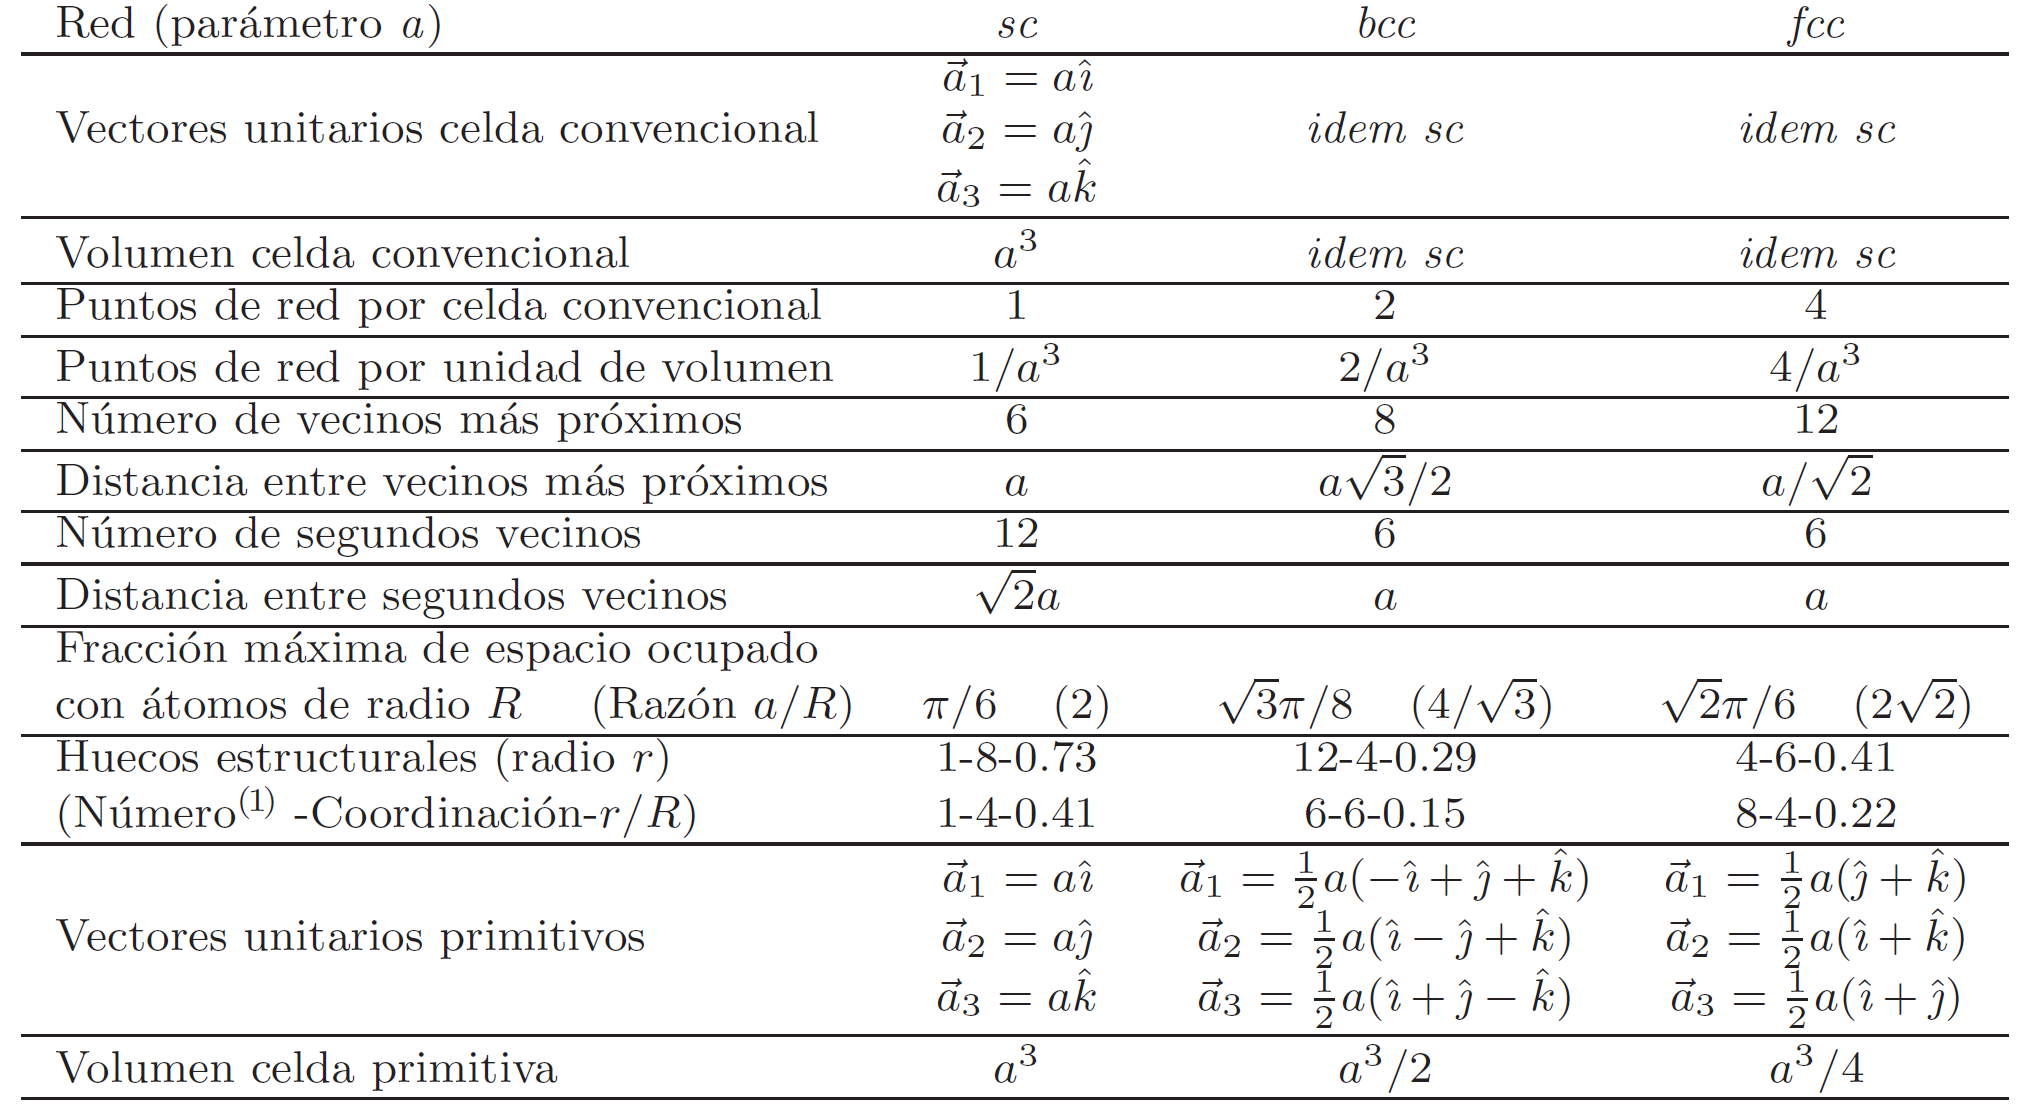
\includegraphics[scale=1.1]{datos.pdf}
\caption{datos experimentales ($I,V_f$) para los 5 filtros.}
\label{Fig:6.0.1}

\end{figure}


\newpage
\subsection{Curvas de corte} \label{Subsec:6.1}

\begin{figure}[h!]  \centering
\includegraphics[scale=0.97]{Datos_cortes_1.pdf}
\caption{aproximación lineal para obtener el punto de corte $\lambda=340$ nm.}
\label{Fig:6.1.1}
\end{figure}

\begin{figure}[h!]  \centering
\includegraphics[scale=0.97]{Datos_cortes_2.pdf}
\caption{aproximación lineal para obtener el punto de corte $\lambda=405$ nm.}
\label{Fig:6.1.2}
\end{figure}

\newpage
\begin{figure}[h!]  \centering
\includegraphics[scale=0.97]{Datos_cortes_3.pdf}
\caption{aproximación lineal para obtener el punto de corte $\lambda=436$ nm.}
\label{Fig:6.1.3}
\end{figure}

\begin{figure}[h!]  \centering
\includegraphics[scale=0.97]{Datos_cortes_4.pdf}
\caption{aproximación lineal para obtener el punto de corte $\lambda=546$ nm.}
\label{Fig:6.1.4}
\end{figure}
\newpage

\begin{figure}[h!]  \centering
\includegraphics[scale=0.97]{Datos_cortes_5.pdf}
\caption{aproximación lineal para obtener el punto de corte $\lambda=580$ nm.}
\label{Fig:6.1.5}
\end{figure}




\subsection{Aproximación exponencial} \label{Subsec:6.2}



\begin{figure}[h!]  \centering
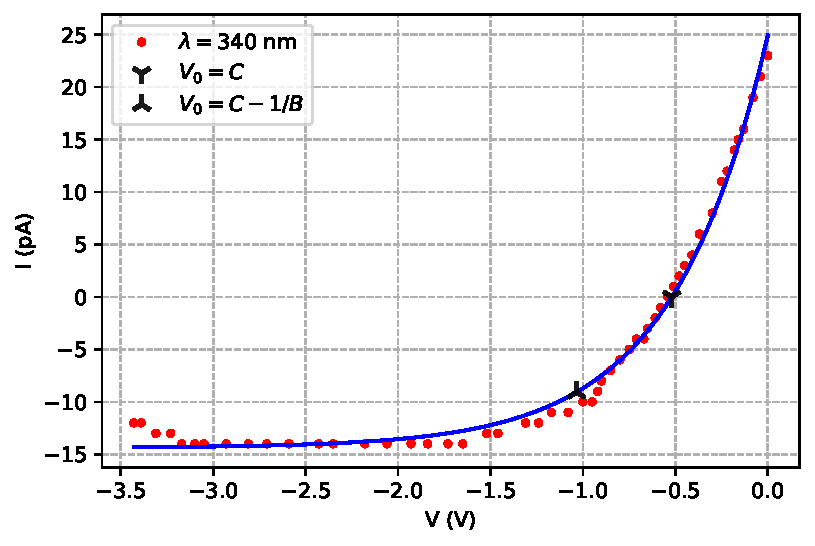
\includegraphics[scale=0.97]{Datos_exponencial_1.pdf}
\caption{aproximación exponencial para obtener el punto de corte $\lambda=340$ nm.}
\label{Fig:6.2.1}
\end{figure}
\newpage
\begin{figure}[h!]  \centering
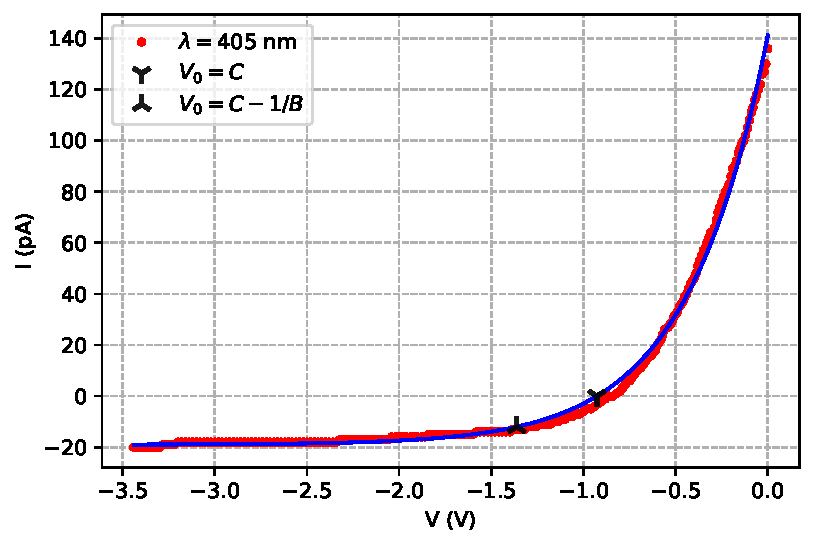
\includegraphics[scale=0.97]{Datos_exponencial_2.pdf}
\caption{aproximación exponencial para obtener el punto de corte $\lambda=405$ nm.}
\label{Fig:6.2.2}
\end{figure}

\begin{figure}[h!]  \centering
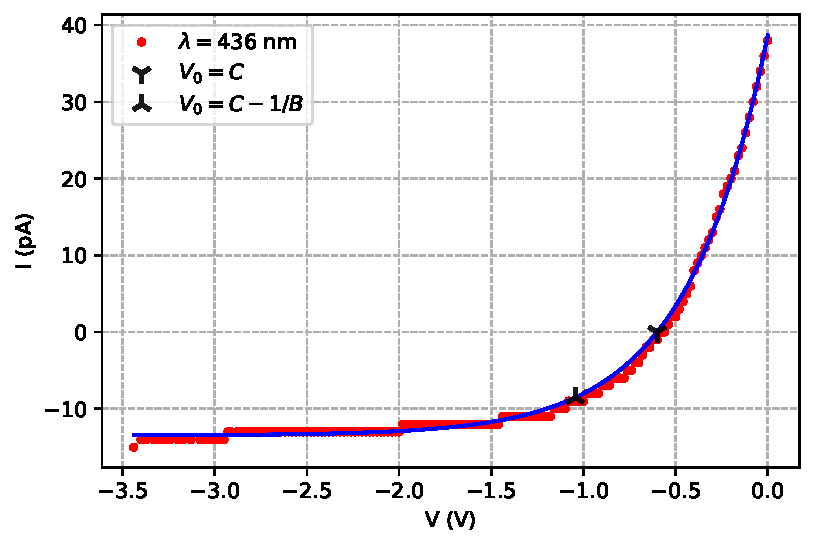
\includegraphics[scale=0.97]{Datos_exponencial_3.pdf}
\caption{aproximación exponencial para obtener el punto de corte $\lambda=436$ nm.}
\label{Fig:6.2.3}
\end{figure}

\newpage
\begin{figure}[h!]  \centering
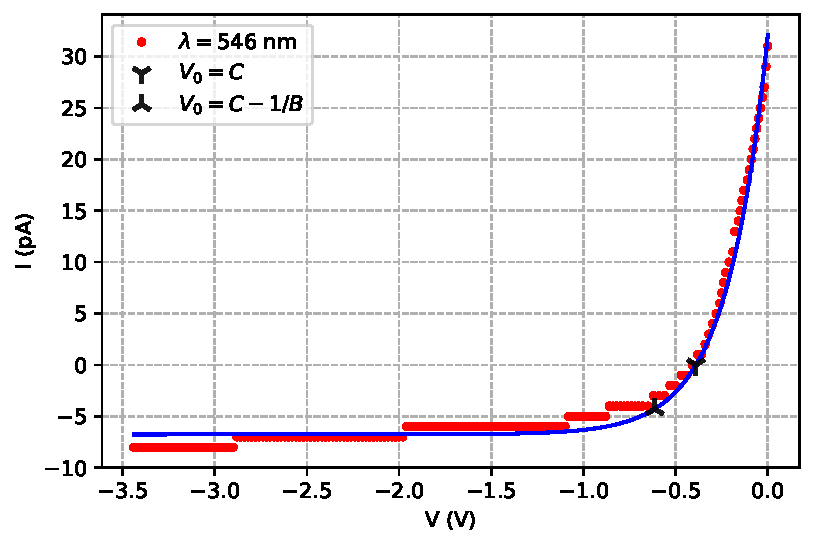
\includegraphics[scale=0.97]{Datos_exponencial_4.pdf}
\caption{aproximación exponencial para obtener el punto de corte $\lambda=546$ nm.}
\label{Fig:6.2.4}
\end{figure}

\begin{figure}[h!]  \centering
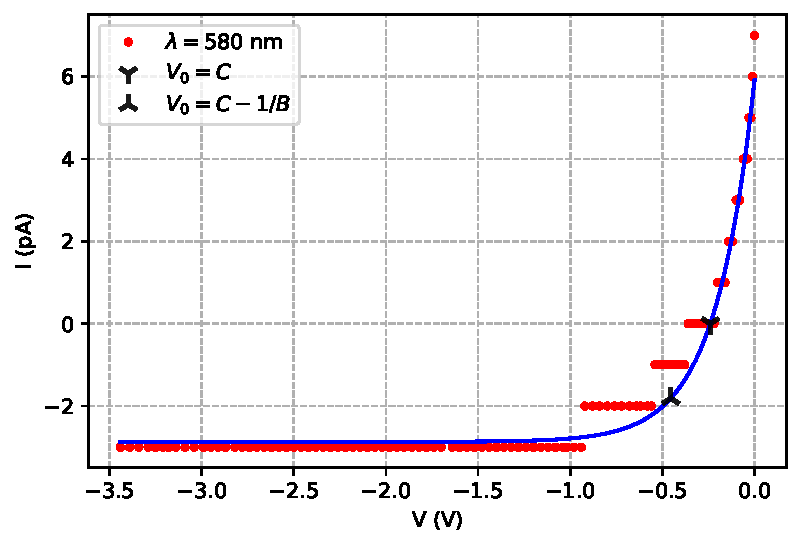
\includegraphics[scale=0.97]{Datos_exponencial_5.pdf}
\caption{aproximación exponencial para obtener el punto de corte $\lambda=580$ nm.}
\label{Fig:6.2.5}
\end{figure}
\subsection{Primer método}

\newpage

\begin{figure}[h!]  \centering
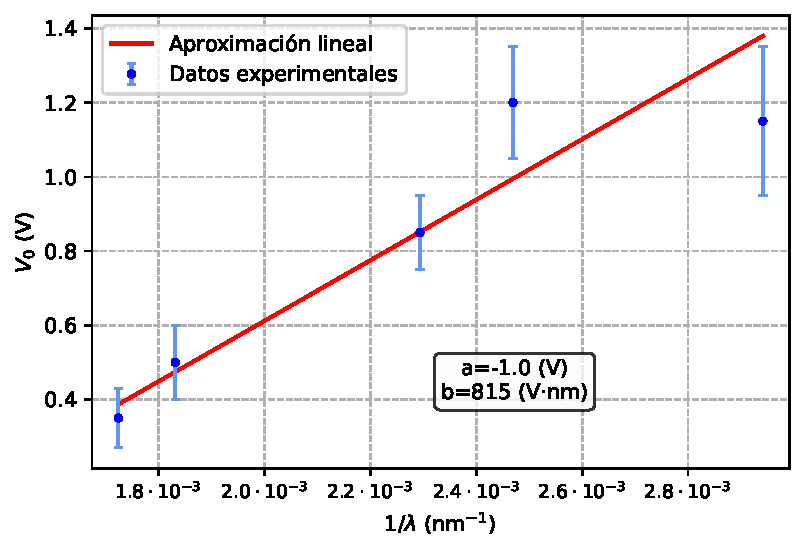
\includegraphics[scale=0.97]{Metodo_1-con.pdf}
\caption{regresión lineal de $V_0$ y $1/\lambda$ con el primer filtro.}
\label{Fig:6.3.1}
\end{figure}

\begin{figure}[h!]  \centering
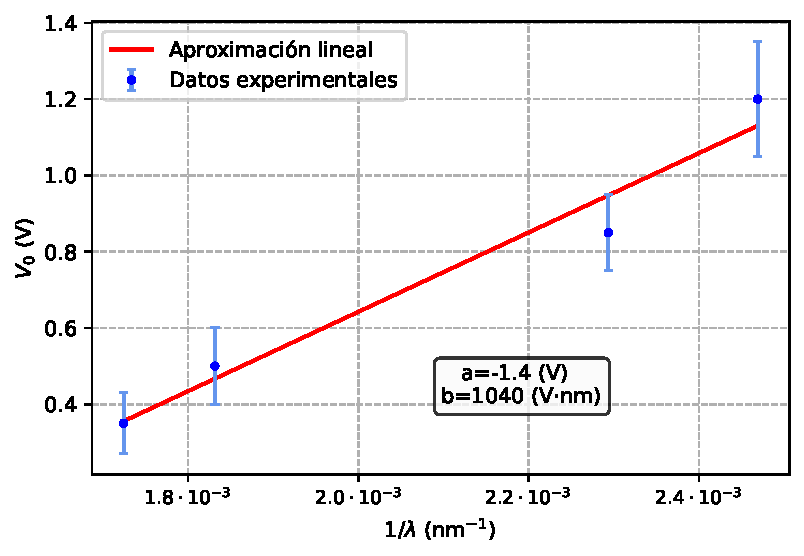
\includegraphics[scale=0.97]{Metodo_1-sin.pdf}
\caption{regresión lineal de $V_0$ y $1/\lambda$ sin el primer filtro.}
\label{Fig:6.3.2}
\end{figure}

\newpage
\subsection{Segundo método}

\begin{figure}[h!]  \centering
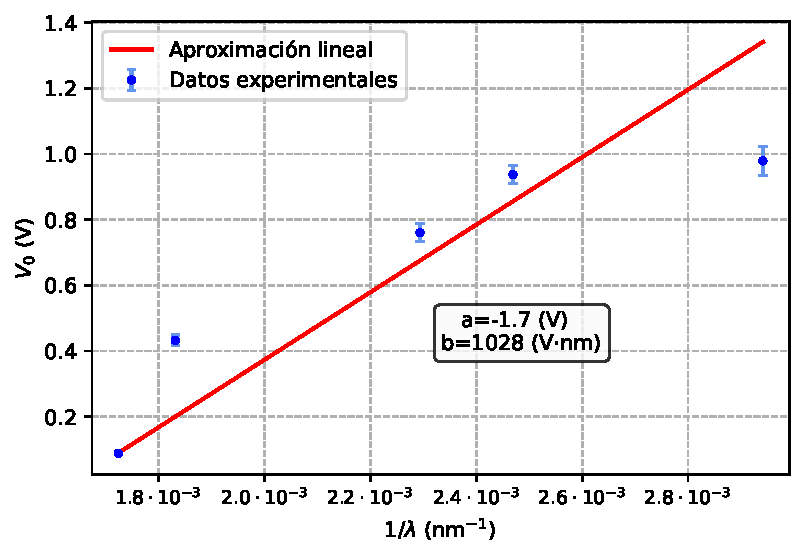
\includegraphics[scale=0.97]{Metodo_2-con.pdf}
\caption{regresión lineal de $V_0$ y $1/\lambda$ con el primer filtro.}
\label{Fig:6.4.1}
\end{figure}

\begin{figure}[h!]  \centering
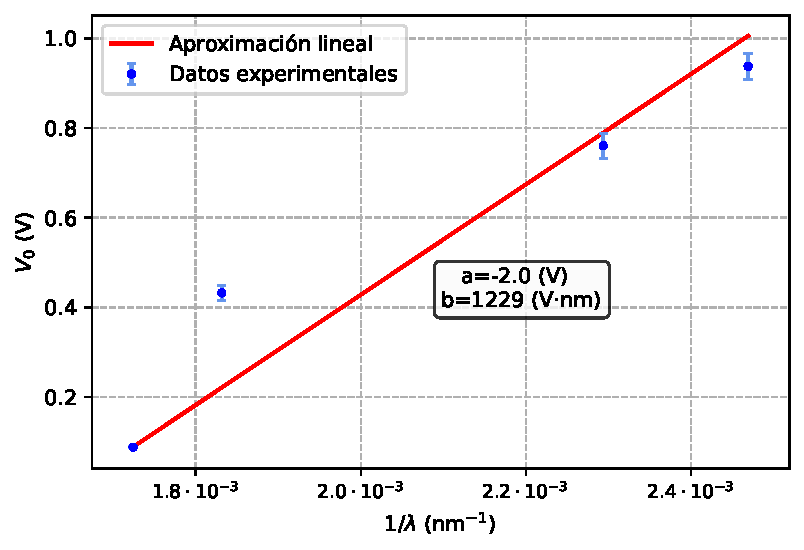
\includegraphics[scale=0.97]{Metodo_2-sin.pdf}
\caption{regresión lineal de $V_0$ y $1/\lambda$ sin el primer filtro.}
\label{Fig:6.4.2}
\end{figure}
\newpage

\subsection{Tercer método}

\subsubsection{Versión tradicional}

\begin{figure}[h!]  \centering
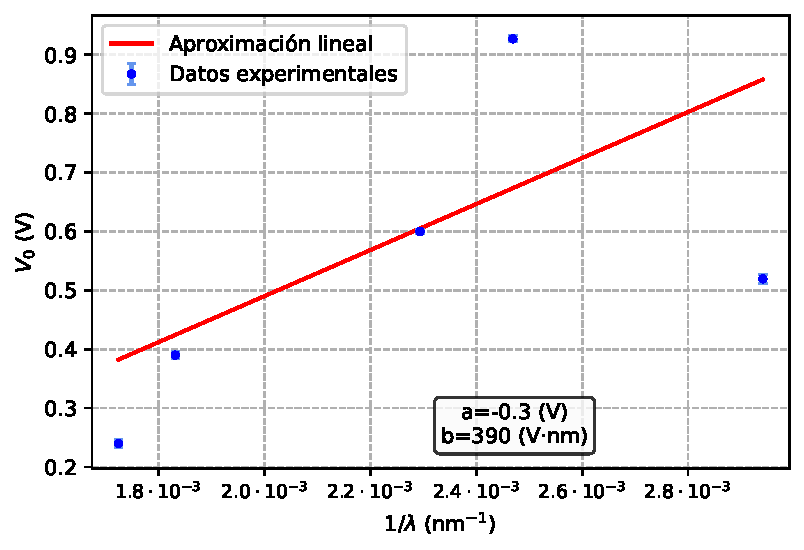
\includegraphics[scale=0.97]{Metodo_3-Clasico-con.pdf}
\caption{regresión lineal de $V_0$ y $1/\lambda$ con el primer filtro.}
\label{Fig:6.5.1}
\end{figure}


\begin{figure}[h!]  \centering
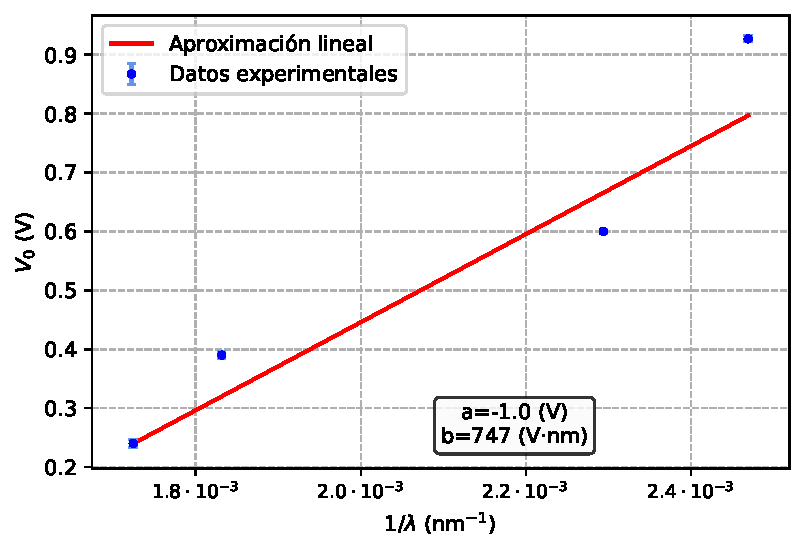
\includegraphics[scale=0.97]{Metodo_3-Clasico-sin.pdf}
\caption{regresión lineal de $V_0$ y $1/\lambda$ sin el primer filtro.}
\label{Fig:6.5.2}
\end{figure}
\newpage

\subsubsection{Nueva versión}

\begin{figure}[h!]  \centering
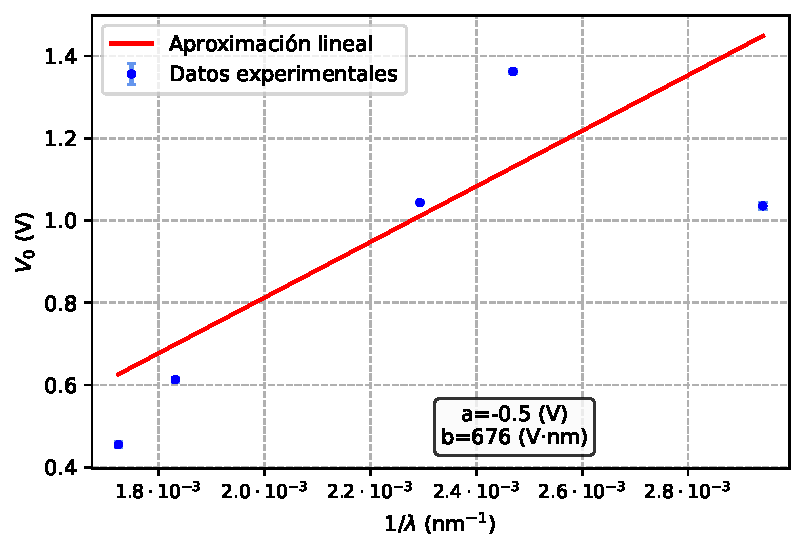
\includegraphics[scale=0.97]{Metodo_3-Nuevo-con.pdf}
\caption{regresión lineal de $V_0$ y $1/\lambda$ con el primer filtro.}
\label{Fig:6.5.3}
\end{figure}

\begin{figure}[h!]  \centering
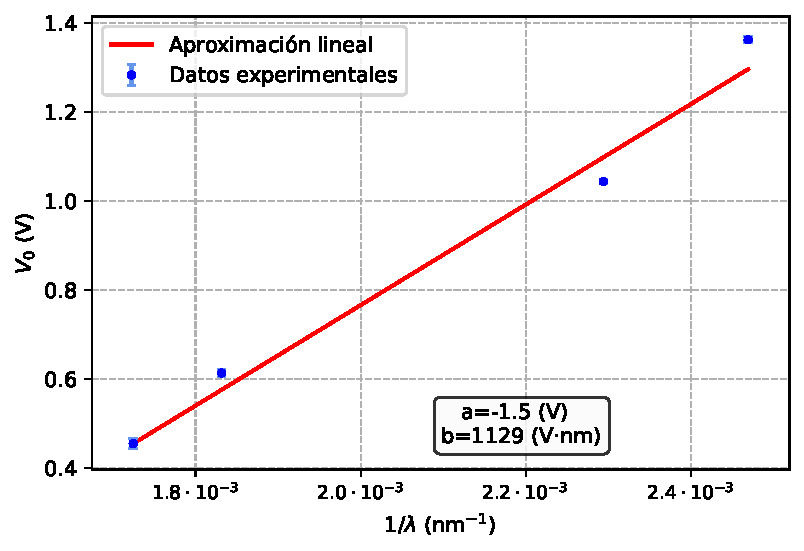
\includegraphics[scale=0.97]{Metodo_3-Nuevo-sin.pdf}
\caption{regresión lineal de $V_0$ y $1/\lambda$ sin el primer filtro.}
\label{Fig:6.5.4}
\end{figure}



\newpage


\section{Datos}  \label{Sec:7-tablas}

\subsection{Potenciales de frenado} \label{Subsec:7.1}


\begin{table}[h!] \centering 
\begin{tabular}{c|c|c} 
 & $V_0$ (V) & $s(V_0)$ (V) \\ \hline 
Metodo 1 & 1.15 &  0.20 \\ 
Metodo 2 & 0.979 &  0.044 \\ 
Metodo 3-1 & 0.5193 &  0.0077 \\ 
Metodo 3-2 & 1.035 &  0.016 \\ \hline
\end{tabular}
\caption{tabla de valores de $V_0$ para $\lambda=340$ nm} 
\label{Tab:7.2.1} 
\end{table} 


\begin{table}[h!] \centering 
\begin{tabular}{c|c|c} 
 & $V_0$ (V) & $s(V_0)$ (V) \\ \hline 
Metodo 1 & 1.20 &  0.15 \\ 
Metodo 2 & 0.937 &  0.028 \\ 
Metodo 3-1 & 0.9269 &  0.0051 \\ 
Metodo 3-2 & 1.3621 &  0.0062 \\ \hline
\end{tabular}
\caption{tabla de valores de $V_0$ para $\lambda=405$ nm} 
\label{Tab:7.2.2} 
\end{table} 

 
\begin{table}[h!] \centering 
\begin{tabular}{c|c|c} 
 & $V_0$ (V) & $s(V_0)$ (V) \\ \hline 
Metodo 1 & 0.85 &  0.10 \\ 
Metodo 2 & 0.760 &  0.028 \\ 
Metodo 3-1 & 0.6000 &  0.0031 \\ 
Metodo 3-2 & 1.0435 &  0.0048 \\ \hline
\end{tabular}
\caption{tabla de valores de $V_0$ para $\lambda=436$ nm} 
\label{Tab:7.2.3} 
\end{table} 


\begin{table}[h!] \centering 
\begin{tabular}{c|c|c} 
 & $V_0$ (V) & $s(V_0)$ (V) \\ \hline 
Metodo 1 & 0.50 &  0.10 \\ 
Metodo 2 & 0.432 &  0.016 \\ 
Metodo 3-1 & 0.3900 &  0.0061 \\ 
Metodo 3-2 & 0.6132 &  0.0076 \\ \hline
\end{tabular}
\caption{tabla de valores de $V_0$ para $\lambda=546$ nm} 
\label{Tab:7.2.4} 
\end{table} 

\newpage

 
\begin{table}[h!] \centering 
\begin{tabular}{c|c|c} 
 & $V_0$ (V) & $s(V_0)$ (V) \\ \hline 
Metodo 1 & 0.350 &  0.080 \\ 
Metodo 2 & 0.0884 &  0.0017 \\ 
Metodo 3-1 & 0.2400 &  0.0073 \\ 
Metodo 3-2 & 0.455 &  0.018 \\ \hline
\end{tabular}
\caption{tabla de valores de $V_0$ para $\lambda=580$ nm \\}  
\label{Tab:7.2.5} 
\end{table}  



\subsection{Constantes $h, \mu_0$ y $W_0$} \label{Subsec:7.2}

\begin{table}[h!] \centering 
\renewcommand{\arraystretch}{1.3} % Ajusta el espacio interlineal
\begin{tabular}{c|c|c|c|c}  
 & $h_1$ (J$\cdot$s) & $s(h_1)$ (J$\cdot$s) & $h_2$ (J$\cdot$s) & $s(h_2)$ (J$\cdot$s) \\ \hline 
Metodo 1 & 4.36 $\cdot 10^{-34}$ & 0.78 $\cdot 10^{-34}$ & 5.26 $\cdot 10^{-34}$ & 0.70 $\cdot 10^{-34}$ \\ 
Metodo 2 & 5.50 $\cdot 10^{-34}$ & 1.20 $\cdot 10^{-34}$ & 6.57 $\cdot 10^{-34}$ & 1.47 $\cdot 10^{-34}$ \\ 
Metodo 3-1 & 2.09 $\cdot 10^{-34}$ & 1.52 $\cdot 10^{-34}$ & 4.00 $\cdot 10^{-34}$ & 1.23 $\cdot 10^{-34}$ \\ 
Metodo 3-2 & 4.59 $\cdot 10^{-34}$ & 1.55 $\cdot 10^{-34}$ & 6.04 $\cdot 10^{-34}$ & 0.78 $\cdot 10^{-34}$ \\ \hline
\end{tabular}\caption{tabla de las constantes de Planck para cada método.} 
\label{Tab:7.3.1} 
\end{table} 

 
\begin{table}[h!] \centering 
\renewcommand{\arraystretch}{1.1} % Ajusta el espacio interlineal
\begin{tabular}{c|c|c|c|c} 
 & $W_1$ (eV) & $s(W_1)$ (eV) & $W_2$ (eV) & $s(W_2)$ (eV) \\ \hline 
Metodo 1  & 1.02  & 0.30 & 1.34  & 0.26  \\ 
Metodo 2  & 1.68  & 0.39 & 2.03  & 0.47  \\ 
Metodo 3-1  & 0.29  & 0.65 & 1.05  & 0.51  \\ 
Metodo 3-2  & 0.92  & 0.66 & 1.49  & 0.33  \\  \hline
\end{tabular}
\caption{tabla de la función de trabajo para cada método.} 
\label{Tab:7.3.2} 
\end{table} 

\begin{table}[h!] \centering 
\renewcommand{\arraystretch}{1.3} % Ajusta el espacio interlineal
\begin{tabular}{c|c|c|c|c} 
 & $\nu_{0_1}$ (Hz) & $s(\nu_{0_1})$ (Hz) & $\nu_{0_2}$ (Hz) & $s(\nu_{0_2})$ (Hz) \\ \hline 
Metodo 1 & 3.75 $\cdot 10^{14}$ & 1.19 $\cdot 10^{14}$ & 4.08 $\cdot 10^{14}$ & 0.97 $\cdot 10^{14}$ \\ 
Metodo 2 & 4.91 $\cdot 10^{14}$ & 1.35 $\cdot 10^{14}$ & 4.95 $\cdot 10^{14}$ & 1.60 $\cdot 10^{14}$ \\ 
Metodo 3-1 & 2.24 $\cdot 10^{14}$ & 5.00 $\cdot 10^{14}$ & 4.21 $\cdot 10^{14}$ & 2.43 $\cdot 10^{14}$ \\ 
Metodo 3-2 & 3.21 $\cdot 10^{14}$ & 2.38 $\cdot 10^{14}$ & 3.96 $\cdot 10^{14}$ & 1.00 $\cdot 10^{14}$ \\  \hline
\end{tabular}
\caption{tabla de la frecuencia umbral para cada método.} 
\label{Tab:7.3.3} 
\end{table} 




\newpage 


\begin{thebibliography}{n}
\bibitem{libro-1} Luis Miguel Varela Cabo; Faustino Gomez, Jesus Carrete;
{\it Tratamiento de datos físicos}.
\bibitem{paper-2} Varios autores; {\it Guiones Técnicas III Física cuántica}
Universidad de Santiago de Compostela.

\end{thebibliography}

\end{document}